\documentclass[tikz, border=10pt]{standalone}

% Pacote necessário para o \mathbb{R}
\usepackage{amssymb}
\usepackage{amsmath}

\usepackage{tikz}
\usetikzlibrary{
    positioning,
    arrows.meta,
    shapes.geometric,
    fit,
    backgrounds
}

\begin{document}

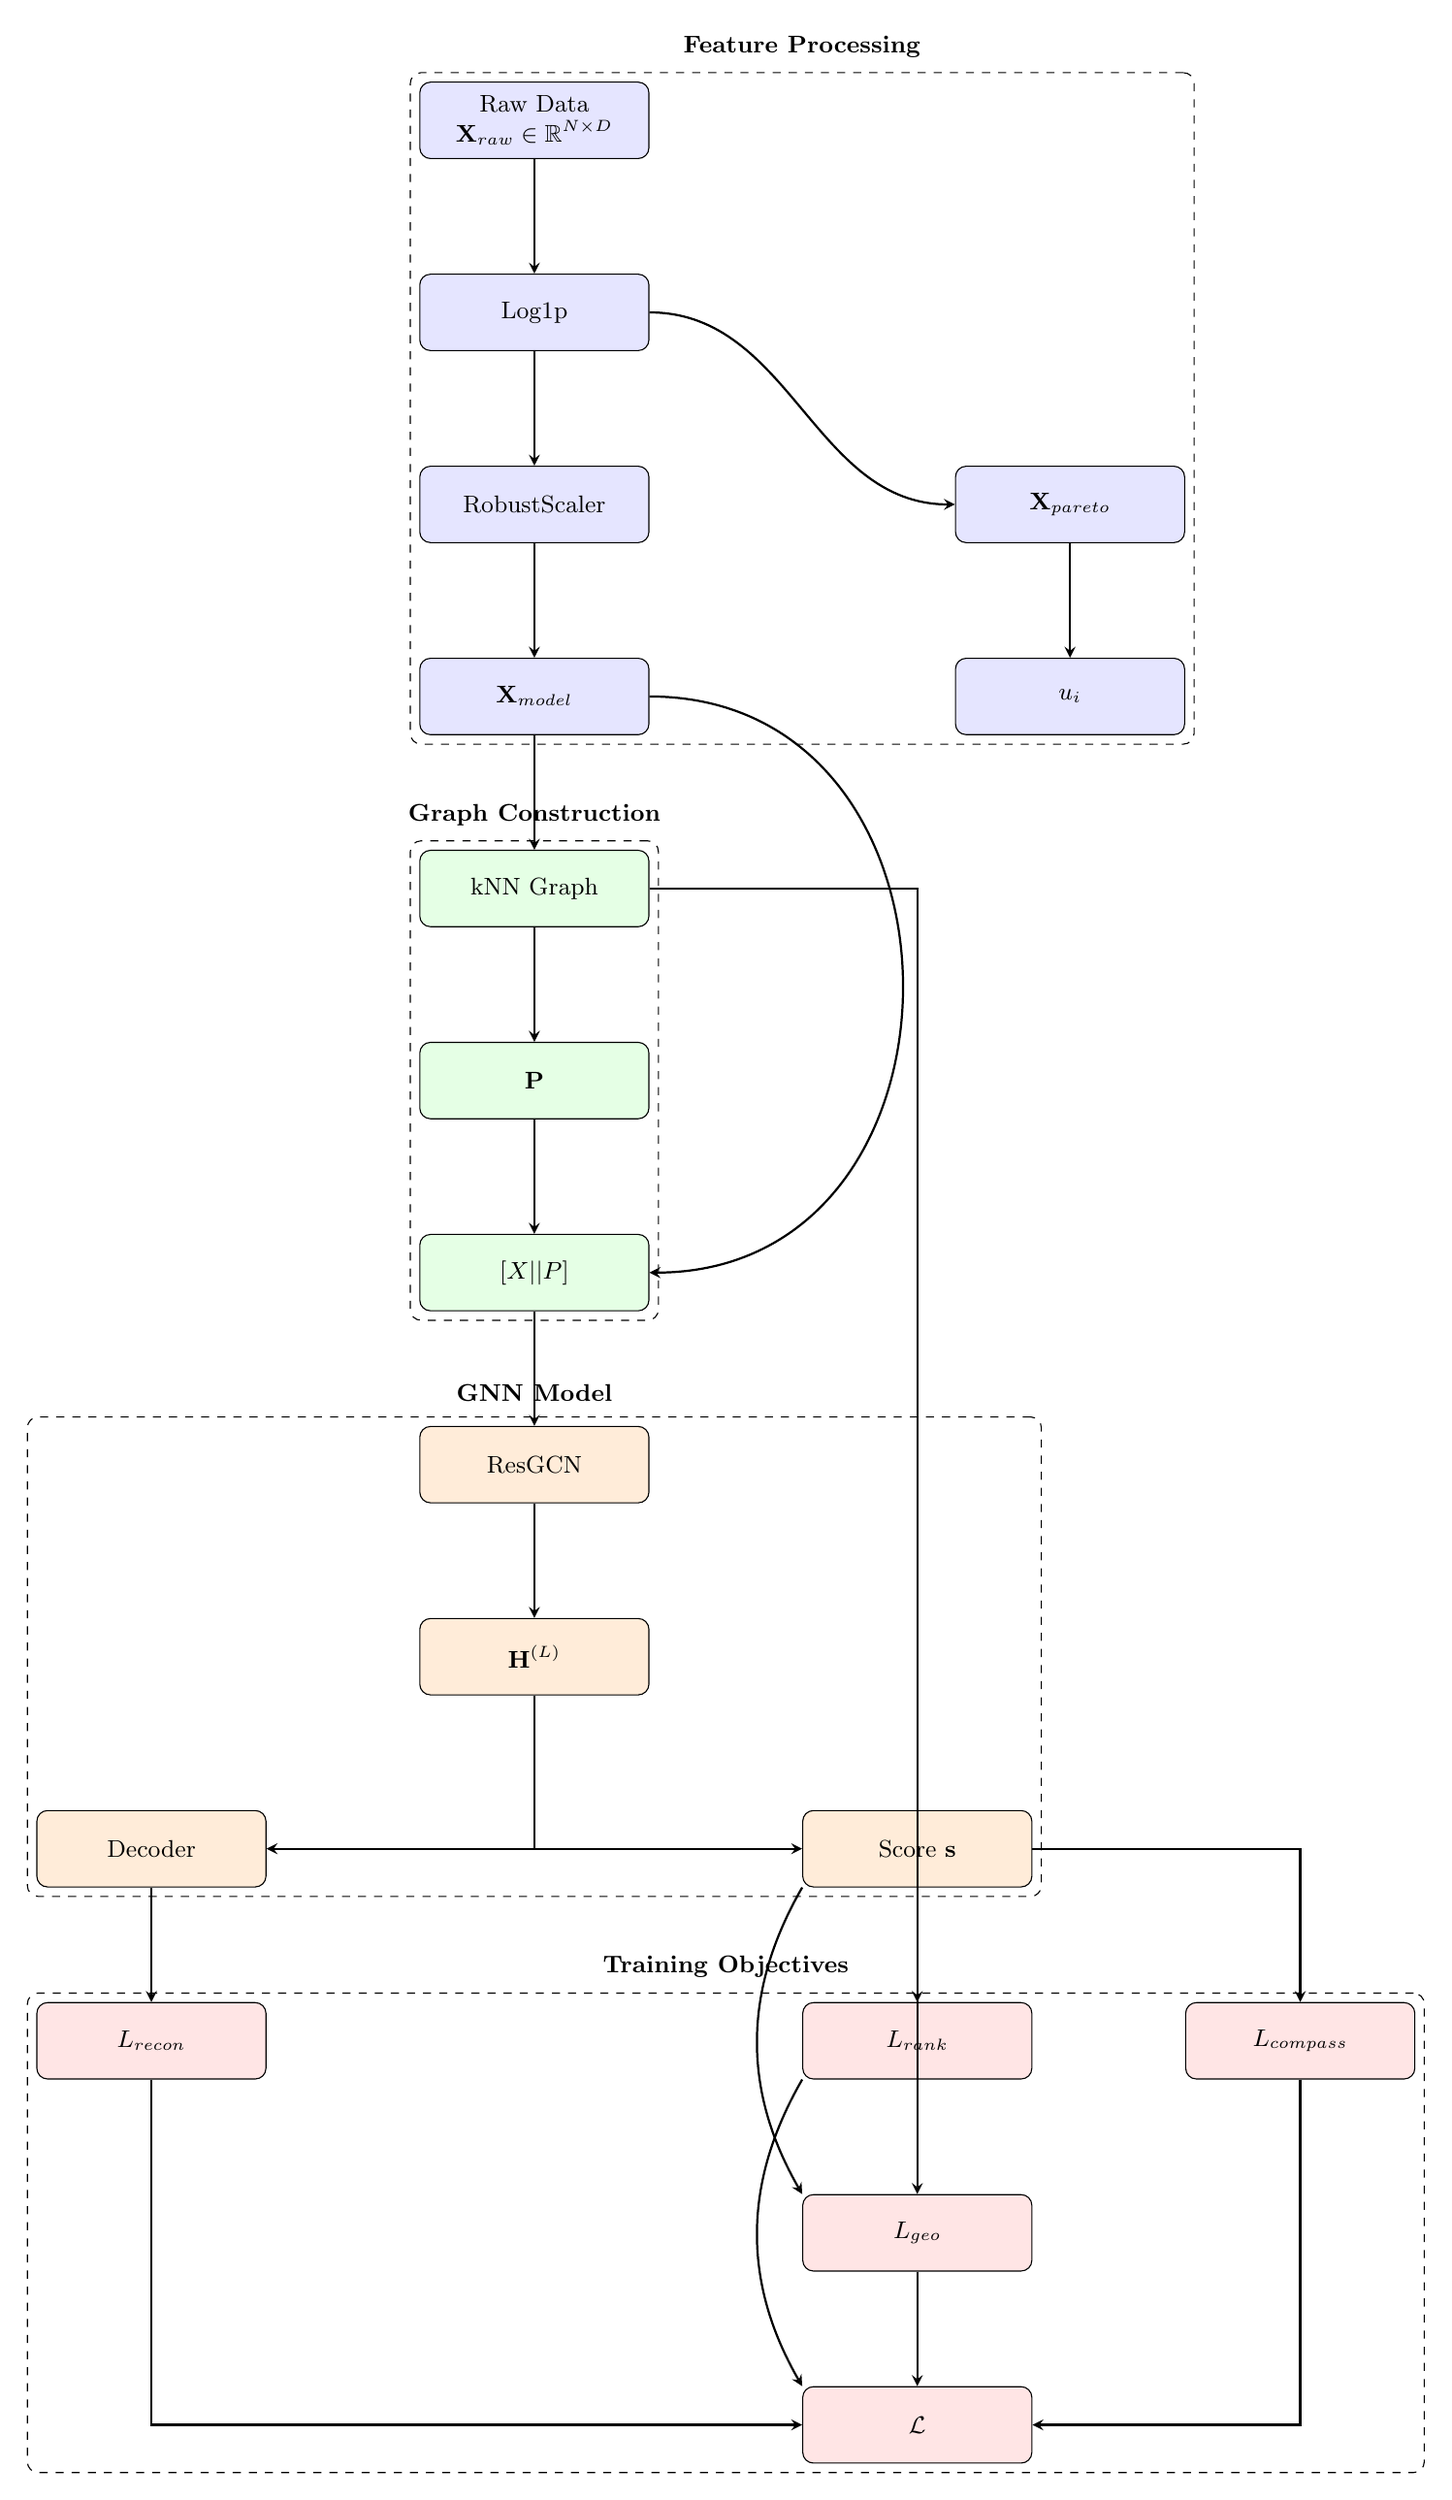
\begin{tikzpicture}[
    node distance=1.5cm and 2cm,
    every node/.style={font=\small},
    block/.style={rectangle, draw, rounded corners, align=center, minimum width=3cm, minimum height=1cm},
    data/.style={block, fill=blue!10},
    graph/.style={block, fill=green!10},
    model/.style={block, fill=orange!15},
    loss/.style={block, fill=red!10},
    arrow/.style={->, thick, >=stealth}
]

% ================= DATA =================
\node[data] (raw) {Raw Data \\ $\mathbf{X}_{raw} \in \mathbb{R}^{N \times D}$};
\node[data, below=of raw] (log) {Log1p};
\node[data, below=of log] (robust) {RobustScaler};
\node[data, below=of robust] (std) {$\mathbf{X}_{model}$};

\node[data, right=4cm of robust] (minmax) {$\mathbf{X}_{pareto}$};
\node[data, below=of minmax] (proxy) {$u_i$};

% ================= GRAPH =================
\node[graph, below=of std] (knn) {kNN Graph};
\node[graph, below=of knn] (posenc) {$\mathbf{P}$};
\node[graph, below=of posenc] (concat) {$[X||P]$};

% ================= MODEL =================
\node[model, below=of concat] (gnn1) {ResGCN};
\node[model, below=of gnn1] (gnn2) {$\mathbf{H}^{(L)}$};

\node[model, below left=of gnn2] (decoder) {Decoder};
\node[model, below right=of gnn2] (ranker) {Score $\mathbf{s}$};

% ================= LOSSES =================
\node[loss, below=of decoder] (reconloss) {$L_{recon}$};
\node[loss, below=of ranker] (rankloss) {$L_{rank}$};
\node[loss, right=of rankloss] (comploss) {$L_{compass}$};
\node[loss, below=of rankloss] (geoloss) {$L_{geo}$};
\node[loss, below=of geoloss] (total) {$\mathcal{L}$};

% ================= ARROWS =================
\draw[arrow] (raw) -- (log);
\draw[arrow] (log) -- (robust);
\draw[arrow] (robust) -- (std);

% Ajustado para uma curva suave S
\draw[arrow] (log.east) to[out=0, in=180] (minmax.west);
\draw[arrow] (minmax) -- (proxy);

\draw[arrow] (std) -- (knn);
\draw[arrow] (knn) -- (posenc);
\draw[arrow] (posenc) -- (concat);

% Ajustado para fazer uma curva lateral em vez de cruzar a caixa
\draw[arrow] (std.east) to[out=0, in=0, looseness=1.5] (concat.east);

\draw[arrow] (concat) -- (gnn1);
\draw[arrow] (gnn1) -- (gnn2);

\draw[arrow] (gnn2) |- (decoder);
\draw[arrow] (gnn2) |- (ranker);

\draw[arrow] (decoder) -- (reconloss);
\draw[arrow] (ranker) -- (rankloss);

\draw[arrow] (ranker.east) -| (comploss.north);

% Setas curvadas para evitar que passem por cima dos nós do meio
\draw[arrow] (ranker.south west) to[bend right=30] (geoloss.north west);
\draw[arrow] (rankloss.south west) to[bend right=30] (total.north west);

\draw[arrow] (knn.east) -| (geoloss.north);

\draw[arrow] (reconloss) |- (total);
\draw[arrow] (comploss) |- (total);
\draw[arrow] (geoloss) -- (total);

% ================= GROUP BOXES =================
\begin{scope}[on background layer]

\node[draw, dashed, rounded corners, fit=(raw)(std)(minmax)(proxy)]
      (group1) {};
\node[above=2pt of group1] {\textbf{Feature Processing}};

\node[draw, dashed, rounded corners, fit=(knn)(posenc)(concat)]
      (group2) {};
\node[above=2pt of group2] {\textbf{Graph Construction}};

\node[draw, dashed, rounded corners, fit=(gnn1)(gnn2)(decoder)(ranker)]
      (group3) {};
\node[above=2pt of group3] {\textbf{GNN Model}};

\node[draw, dashed, rounded corners, fit=(reconloss)(rankloss)(comploss)(geoloss)(total)]
      (group4) {};
\node[above=2pt of group4] {\textbf{Training Objectives}};

\end{scope}

\end{tikzpicture}

\end{document}